
% This LaTeX was auto-generated from an M-file by MATLAB.
% To make changes, update the M-file and republish this document.

\documentclass{article}
\usepackage{graphicx}
\usepackage{color}

\sloppy
\definecolor{lightgray}{gray}{0.5}
\setlength{\parindent}{0pt}

\begin{document}

    
    

\section*{Wireless Comms Mini Matlab 1}

\begin{verbatim}
%Neema Aggarwal
%Shivam Mevawala
%Nicobitch

close all;
rate=0; % if rate is 1, then puncture, making code rate 3/4

SNR = -4:1:8; %list of SNR values to run algorithm
%intialize vecs
BERc=zeros(length(SNR));
tblen =32; %will handle delay for convolution coder

n=3072; %msg length, must be mult of 6,4, and 128
m=4; %QPSK is 4-QAM
punc= [1 1 1 0 0 1]; %drops two bits out of ever 6
nsubc=128; % number of subcarriers

if rate
    coderate = 3/4;
else
    coderate = 1/2;
end
%use the SNR to calculate EbNo
EbNo_c = SNR -10*log10(log2(m)*coderate);

%loop over SNR values
for k=1:length(SNR)
X=randi([0 m-1],1,n);
%convert symbols to binary
X_bin = reshape((de2bi(X, 2,'left-msb')).',1,n*2);
%define a trellis (default chosen) with coderate 1/2 (puncture will take
%care of converting to 3/4 coderate)
trellis = poly2trellis(7,[171 133]);
%encode (based on which coderate we want)
if rate
    code = convenc(X_bin,trellis, punc);
else
    code = convenc(X_bin,trellis);
end
%modulate
Yc=qammod(bin2dec([num2str(code(1:2:end-1)') num2str(code(2:2:end)')])',m);

% parallelize
Pc=zeros(length(Yc)/128,128);
for kk=1:length(Yc)/128
Pc(kk,:)=Yc(1,((kk-1)*128+1):((kk)*128));
end
% IFFT
ifft_sig=ifft(Pc',nsubc)';

% Adding Cyclic Extension to enable circular conv

cext_data=zeros(length(Yc)/128,nsubc+32);
cext_data(:,(1:32))=ifft_sig(:,(nsubc-31:nsubc));
for i=1:nsubc

    cext_data(:,(i+32))=ifft_sig(:,i);

end

%add noise
Ac=awgn(cext_data, SNR(k),'measured');

%Removing Cyclic Extension
rxed_sig=zeros(length(Yc)/128,nsubc);
for i=1:nsubc
    rxed_sig(:,i)=Ac(:,i+32);
end


% FFT
ff_sig=fft(rxed_sig',nsubc)';

%serialize
Sc=zeros(1,length(Yc));

for kkk=1:length(Yc)/128

    Sc((kkk-1)*128+1:(kkk)*128)=ff_sig(kkk,:);
end

%demodulate
Zc=reshape(de2bi(qamdemod(Sc,m),2,'left-msb').',1,length(Sc)*2);
%decode based on coderate
if rate
    d = vitdec(Zc,trellis,tblen,'trunc','hard', punc);
else
    d = vitdec(Zc,trellis,tblen,'trunc','hard');
end
%calculate bit error rate
ber=biterr(d,X_bin)/(2*n);
BERc(k)=ber;
end

% plot theoretical and actual BER
figure
SPECT = distspec(trellis,7);
semilogy(EbNo_c,bercoding(EbNo_c, 'conv', 'hard', 1/2, SPECT),'m-');
hold on;
semilogy(EbNo_c, BERc,'kx');

xlabel('EbNo (dB)')
ylabel('BER')
title('Waterfall Plots (Convolutional Coder)')
legend('theoretical', 'actual')
\end{verbatim}
\begin{figure}[H]
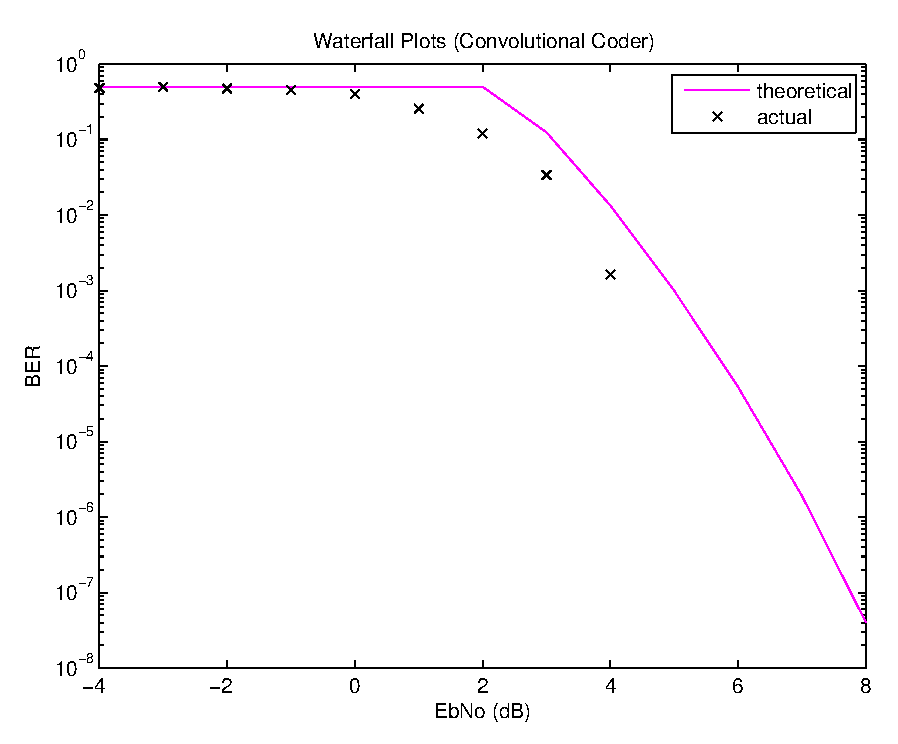
\includegraphics [width=4in]{wireless_sim_01.eps}
\caption{"1/2 code rate"}
\end{figure}
\begin{figure}[H]
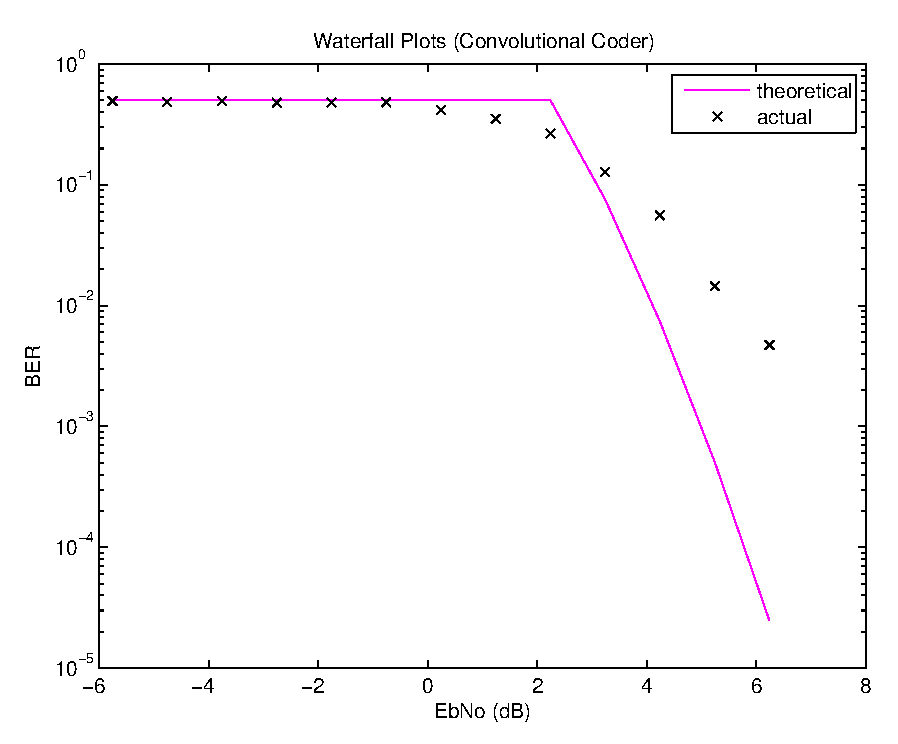
\includegraphics [width=4in]{wireless_sim_four.eps}
\caption{"3/4 code rate"}
\end{figure}

\end{document}
    
